\documentclass{article}

% content/resources/templates/preamble.tex
\usepackage[margin=0.6in]{geometry}
\author{Milav Dabgar}
\usepackage{amsmath,amssymb,amsthm}
\usepackage{booktabs}
\usepackage{multirow}
\usepackage{xcolor}
\usepackage{tcolorbox}
\tcbuselibrary{breakable,skins}
\usepackage[colorlinks=true,linkcolor=blue]{hyperref}
\usepackage{titlesec}
\usepackage{enumitem}
\usepackage{tikz}
\usepackage{pgfplots}
\usepackage{circuitikz}
\usepackage[version=4]{mhchem}
\usepackage{longtable}
\usepackage{array}
\usepackage{float}
\usepackage{caption}
\usepackage{listings}

\lstset{
  basicstyle=\small\ttfamily,
  breaklines=true,
  breakatwhitespace=false,
  postbreak=\mbox{\textcolor{red}{$\hookrightarrow$}\space},
  float=false,
  numbers=left,
  numberstyle=\tiny\color{gray},
  numbersep=10pt,
  xleftmargin=2em,
  keywordstyle=\color{blue},
  commentstyle=\color{green!60!black},
  stringstyle=\color{purple},
  backgroundcolor=\color{gray!5},
  showstringspaces=false,
  tabsize=2,
  captionpos=b,
  keepspaces=true,
  columns=flexible
}

\pgfplotsset{compat=1.18}
\usetikzlibrary{shapes,arrows,positioning,calc,patterns,decorations.pathmorphing,decorations.markings,arrows.meta}

% Color scheme
\definecolor{headcolor}{RGB}{0,102,204}
\definecolor{keycolor}{RGB}{220,20,60}
\definecolor{solutioncolor}{RGB}{34,139,34}
\definecolor{mnemoniccolor}{RGB}{148,0,211}
\definecolor{codecolor}{RGB}{0,0,100}

% Spacing
\setlength{\parskip}{3pt}
\setlist[itemize]{nosep}
\setlist[enumerate]{nosep}

% Title formatting
\titleformat{\section}{\Large\bfseries\color{headcolor}}{\thesection}{1em}{}
\titleformat{\subsection}{\large\bfseries\color{headcolor}}{\thesubsection}{1em}{}

% Pandoc tightlist compatibility
\providecommand{\tightlist}{%
  \setlength{\itemsep}{0pt}\setlength{\parskip}{0pt}}

% Pandoc longtable compatibility
\newcounter{none}
\def\thenone{}


% content/resources/templates/english-boxes.tex
% This file is currently empty - it exists to maintain consistency with the import structure.
% Add custom environments here if needed in the future.


% Custom commands for GTU solutions
% This file defines semantic commands for consistent formatting

% Question command with automatic formatting
\newcommand{\question}[2]{%
  \section*{Question #1}%
  \textbf{#2}%
}

% OR question variant
\newcommand{\questionor}[2]{%
  \section*{Question #1 OR}%
  \textbf{#2}%
}

% Proper table environment with caption
\newenvironment{answertable}[1]{%
  \begin{table}[htbp]
  \centering
  \caption{#1}
}{%
  \end{table}
}

% Proper figure environment for diagrams
\newenvironment{answerdiagram}[1]{%
  \begin{figure}[htbp]
  \centering
  \caption{#1}
}{%
  \end{figure}
}

% Semantic markup for key terms
\newcommand{\keyword}[1]{\textbf{#1}}
\newcommand{\code}[1]{\texttt{#1}}
\newcommand{\classname}[1]{\texttt{#1}}
\newcommand{\methodname}[1]{\texttt{#1}}

% Proper quotation marks
\newcommand{\mnemonic}[1]{``#1''}


\title{Fundamentals of Electrical Engineering (4311101) - Summer 2024 Solution}
\date{June 15, 2024}

\begin{document}
\maketitle

\questionmarks{1(a)}{3}{Define EMF, electric current and power. Also write their units.}

\begin{solutionbox}
\textbf{Answer}:

\begin{center}
\captionof{table}{Definitions and Units}
\begin{tabulary}{\linewidth}{|L|L|L|}
\hline
\textbf{Term} & \textbf{Definition} & \textbf{Unit} \\ \hline
\textbf{EMF (Electromotive Force)} & The energy supplied by a source per unit charge & Volt (V) \\ \hline
\textbf{Electric Current} & The rate of flow of electric charge & Ampere (A) \\ \hline
\textbf{Power} & The rate at which electrical energy is transferred & Watt (W) \\ \hline
\end{tabulary}
\end{center}
\end{solutionbox}

\begin{mnemonicbox}
\mnemonic{EVA: EMF in Volts, Current in Amperes, Power in Watts}
\end{mnemonicbox}

\questionmarks{1(b)}{4}{Three resistors having resistances of 1000 $\Omega$, 2000 $\Omega$ and 3000 $\Omega$ respectively are connected in series. Find the equivalent resistance of this series connection. Now these three resistors are connected in parallel. Find the equivalent resistance of this parallel connection.}

\begin{solutionbox}
\textbf{Answer}:

\textbf{For Series Connection:}
\begin{align*}
R_{eq} &= R_1 + R_2 + R_3 \\
R_{eq} &= 1000 \Omega + 2000 \Omega + 3000 \Omega \\
R_{eq} &= 6000 \Omega
\end{align*}

\textbf{For Parallel Connection:}
\begin{align*}
\frac{1}{R_{eq}} &= \frac{1}{R_1} + \frac{1}{R_2} + \frac{1}{R_3} \\
\frac{1}{R_{eq}} &= \frac{1}{1000} + \frac{1}{2000} + \frac{1}{3000} \\
\frac{1}{R_{eq}} &= 0.001 + 0.0005 + 0.00033 \\
\frac{1}{R_{eq}} &= 0.00183 \\
R_{eq} &= 545.45 \Omega
\end{align*}

\begin{answerdiagram}{Resistor Connections}
\begin{center}
\begin{circuitikz}[american, scale=0.8, transform shape]
    % Series
    \draw (0,0) node[left]{In} to[R, l=1k$\Omega$] (2,0) to[R, l=2k$\Omega$] (4,0) to[R, l=3k$\Omega$] (6,0) node[right]{Out};
    \node at (3,-1) {Series Connection};

    % Parallel
    \begin{scope}[yshift=-3cm]
    \draw (0,1.5) -- (0,0) -- (6,0) -- (6,1.5);
    \draw (0,1.5) -- (6,1.5);
    \draw (1.5,1.5) to[R, l=1k$\Omega$] (1.5,0);
    \draw (3,1.5) to[R, l=2k$\Omega$] (3,0);
    \draw (4.5,1.5) to[R, l=3k$\Omega$] (4.5,0);
    \node at (0,0.75) [left] {In};
    \node at (6,0.75) [right] {Out};
    \node at (3,-1) {Parallel Connection};
    \end{scope}
\end{circuitikz}
\end{center}
\end{answerdiagram}
\end{solutionbox}

\begin{mnemonicbox}
\mnemonic{Series Sum, Parallel Product/Sum: In series add directly, in parallel take reciprocal sum}
\end{mnemonicbox}

\questionmarks{1(c)}{7}{Write the definition of Resistor, Capacitor and Inductor. Draw their symbols and write their units. Also write the use of each device in electrical circuit.}

\begin{solutionbox}
\textbf{Answer}:

\begin{center}
\captionof{table}{Circuit Components}
\begin{tabulary}{\linewidth}{|L|L|C|L|L|}
\hline
\textbf{Component} & \textbf{Definition} & \textbf{Symbol} & \textbf{Unit} & \textbf{Use in Circuit} \\ \hline
\textbf{Resistor} & A component that opposes the flow of electric current & \begin{circuitikz}[baseline, american, scale=0.5] \draw (0,0.2) to[R] (1,0.2); \end{circuitikz} & Ohm ($\Omega$) & Limits current, divides voltage, generates heat \\ \hline
\textbf{Capacitor} & A component that stores electric charge & \begin{circuitikz}[baseline, american, scale=0.5] \draw (0,0.2) to[C] (1,0.2); \end{circuitikz} & Farad (F) & Blocks DC, passes AC, energy storage, filtering \\ \hline
\textbf{Inductor} & A component that stores energy in magnetic field & \begin{circuitikz}[baseline, american, scale=0.5] \draw (0,0.2) to[L] (1,0.2); \end{circuitikz} & Henry (H) & Blocks AC, passes DC, energy storage, filtering \\ \hline
\end{tabulary}
\end{center}
\end{solutionbox}

\begin{mnemonicbox}
\mnemonic{RCI: Resistor Controls current, Capacitor stores charge, Inductor stores magnetic energy}
\end{mnemonicbox}

\questionmarks{1(c) OR}{7}{State Ohm's law and write the equation of Ohm's law with circuit diagram. Write applications of Ohm's law. Also write the limitation of Ohm's law.}

\begin{solutionbox}
\textbf{Answer}:

\keyword{Ohm's Law:} The current flowing through a conductor is directly proportional to the voltage across it and inversely proportional to its resistance.

\keyword{Equation:} $V = I \times R$

\begin{answerdiagram}{Ohm's Law Circuit}
\begin{circuitikz}[american]
    \draw (0,0) to[V, v=$V$] (0,2) -- (2,2)
          to[R, l=$R$, i=$I$] (2,0) -- (0,0);
\end{circuitikz}
\end{answerdiagram}

\keyword{Applications of Ohm's Law:}
\begin{itemize}
    \item Calculating current, voltage, or resistance in circuits
    \item Designing electrical and electronic circuits
    \item Power calculations ($P = V \times I = I^2 \times R = V^2/R$)
    \item Circuit analysis using voltage divider and current divider
\end{itemize}

\keyword{Limitations of Ohm's Law:}
\begin{itemize}
    \item Not applicable for non-linear devices (diodes, transistors)
    \item Not valid for high-frequency AC circuits
    \item Not valid for non-metallic conductors
    \item Does not apply during transient conditions
\end{itemize}
\end{solutionbox}

\begin{mnemonicbox}
\mnemonic{VIR: Voltage equals current times resistance}
\end{mnemonicbox}

\questionmarks{2(a)}{3}{Explain the generation of alternating EMF with the help of necessary diagram and equation.}

\begin{solutionbox}
\textbf{Answer}:

Alternating EMF is generated when a conductor rotates in a magnetic field.

\keyword{Equation:} $e = E_0 \sin(\omega t) = E_0 \sin(2\pi ft)$

Where:
\begin{itemize}
    \item $e$ = instantaneous EMF
    \item $E_0$ = maximum EMF
    \item $\omega$ = angular velocity ($2\pi f$)
    \item $f$ = frequency
    \item $t$ = time
\end{itemize}

\begin{answerdiagram}{AC Generation Principle}
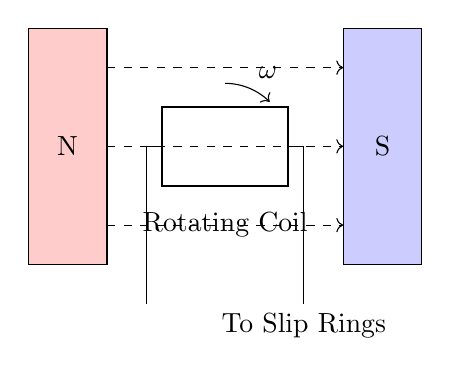
\begin{tikzpicture}
    % Magnetic Poles
    \draw[fill=red!20] (-2.5,-1.5) rectangle (-1.5,1.5) node[midway]{N};
    \draw[fill=blue!20] (1.5,-1.5) rectangle (2.5,1.5) node[midway]{S};
    
    % Field Lines
    \draw[dashed, ->] (-1.5,1) -- (1.5,1);
    \draw[dashed, ->] (-1.5,0) -- (1.5,0);
    \draw[dashed, ->] (-1.5,-1) -- (1.5,-1);
    
    % Coil
    \draw[thick] (-0.8,-0.5) rectangle (0.8,0.5);
    \draw[->] (0,0.8) arc (90:45:0.8) node[midway, above right] {$\omega$};
    \node at (0,-1) {Rotating Coil};
    
    % Connections
    \draw (0.8,0) -- (1,0) -- (1,-2) node[below] {To Slip Rings};
    \draw (-0.8,0) -- (-1,0) -- (-1,-2);
\end{tikzpicture}
\end{answerdiagram}
\end{solutionbox}

\begin{mnemonicbox}
\mnemonic{RCBS: Rotation of Coil in magnetic field produces sinusoidal EMF}
\end{mnemonicbox}

\questionmarks{2(b)}{4}{Explain the behavior of pure capacitor with AC supply with necessary circuit diagram and equation.}

\begin{solutionbox}
\textbf{Answer}:

\keyword{Behavior of Pure Capacitor with AC:}
\begin{itemize}
    \item Current leads voltage by 90$^\circ$ in a pure capacitor
    \item Capacitive reactance ($X_c$) = $1/(2\pi fC)$
    \item As frequency increases, reactance decreases
    \item Stores energy in electric field during charging
\end{itemize}

\begin{answerdiagram}{Capacitor Circuit and Waveform}
\begin{circuitikz}[american, scale=0.8]
    \draw (0,0) to[sinusoidal voltage source, l=AC] (0,2) -- (2,2) to[C, l=C] (2,0) -- (0,0);
\end{circuitikz}
\quad
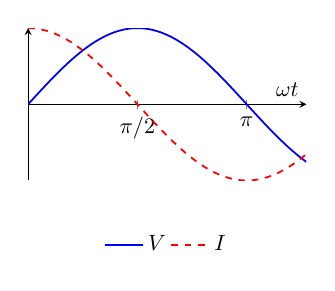
\begin{tikzpicture}[scale=0.8]
    \begin{axis}[
        width=6cm, height=4cm,
        axis lines=middle,
        xtick={0, 1.57, 3.14},
        xticklabels={0, $\pi/2$, $\pi$},
        ytick=\empty,
        xlabel=$\omega t$,
        legend style={at={(0.5,-0.3)}, anchor=north, legend columns=-1, draw=none}
    ]
    \addplot[blue, thick, domain=0:4, samples=100] {sin(deg(x))};
    \addlegendentry{$V$}
    \addplot[red, dashed, thick, domain=0:4, samples=100] {cos(deg(x))};
    \addlegendentry{$I$}
    \end{axis}
\end{tikzpicture}
\end{answerdiagram}

\keyword{Equation:} $I = C \times \frac{dV}{dt}$
\end{solutionbox}

\begin{mnemonicbox}
\mnemonic{CIVIC: Capacitor's current Is ahead of Voltage by 90 In Circuit}
\end{mnemonicbox}

\questionmarks{2(c)}{7}{An AC voltage is expressed as 300 Sin (628t) V. Find (i) Amplitude (ii) Frequency (iii) Time period (iv) Average value (v) RMS Value (vi) Form Factor and (vii) Peak Factor for this AC voltage.}

\begin{solutionbox}
\textbf{Answer}:

Given: $v = 300 \sin(628t)$ V

\begin{center}
\captionof{table}{Calculated Parameters}
\begin{tabulary}{\linewidth}{|L|L|L|L|}
\hline
\textbf{Parameter} & \textbf{Formula} & \textbf{Calculation} & \textbf{Result} \\ \hline
\textbf{Amplitude} & $V_m$ & 300 V & 300 V \\ \hline
\textbf{Angular Frequency} & $\omega$ & 628 rad/s & 628 rad/s \\ \hline
\textbf{Frequency} & $f = \omega/2\pi$ & $628/6.28$ & 100 Hz \\ \hline
\textbf{Time Period} & $T = 1/f$ & $1/100$ & 0.01 s \\ \hline
\textbf{Average Value} & $V_{avg} = 2V_m/\pi$ & $2 \times 300 / 3.14$ & 191 V \\ \hline
\textbf{RMS Value} & $V_{rms} = V_m/\sqrt{2}$ & $300/1.414$ & 212.16 V \\ \hline
\textbf{Form Factor} & $FF = V_{rms}/V_{avg}$ & $212.16/191$ & 1.11 \\ \hline
\textbf{Peak Factor} & $PF = V_m/V_{rms}$ & $300/212.16$ & 1.414 \\ \hline
\end{tabulary}
\end{center}
\end{solutionbox}

\begin{mnemonicbox}
\mnemonic{FART FAFP: Frequency, Angular, RMS, Time; Form factor, Average, Peak factor}
\end{mnemonicbox}

\questionmarks{2(a) OR}{3}{Explain the generation of 3-phase alternating EMF.}

\begin{solutionbox}
\textbf{Answer}:

3-phase alternating EMF is generated using three separate coils placed 120$^\circ$ apart in a magnetic field.

\keyword{Key Points:}
\begin{itemize}
    \item Three identical coils are placed 120$^\circ$ apart
    \item Each coil produces sinusoidal EMF
    \item Phases are labeled as R, Y, and B
    \item Phase difference between any two phases is 120$^\circ$
\end{itemize}

\begin{answerdiagram}{3-Phase Generation}
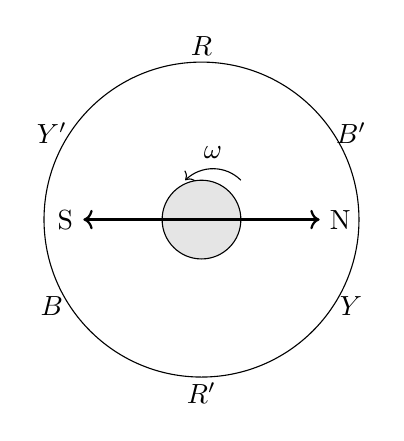
\begin{tikzpicture}
    % Stator
    \draw (0,0) circle (2cm);
    \node at (0,2.2) {$R$};
    \node at (0,-2.2) {$R'$};
    \node at (1.9,1.1) {$B'$};
    \node at (-1.9,-1.1) {$B$};
    \node at (1.9,-1.1) {$Y$};
    \node at (-1.9,1.1) {$Y'$};
    
    % Rotor
    \draw[fill=gray!20] (0,0) circle (0.5cm);
    \draw[->, thick] (0,0) -- (1.5,0) node[right] {N};
    \draw[->, thick] (0,0) -- (-1.5,0) node[left] {S};
    \draw[->] (0.5,0.5) arc (45:135:0.5) node[midway, above] {$\omega$};
\end{tikzpicture}
\end{answerdiagram}
\end{solutionbox}

\begin{mnemonicbox}
\mnemonic{THREE: Three coils Have 120 Rotating EMF Each}
\end{mnemonicbox}

\questionmarks{2(b) OR}{4}{Explain the behavior of pure inductor with AC supply with necessary circuit diagram and equation.}

\begin{solutionbox}
\textbf{Answer}:

\keyword{Behavior of Pure Inductor with AC:}
\begin{itemize}
    \item Current lags voltage by 90$^\circ$ in a pure inductor
    \item Inductive reactance ($X_L$) = $2\pi fL$
    \item As frequency increases, reactance increases
    \item Stores energy in magnetic field
\end{itemize}

\begin{answerdiagram}{Inductor Circuit and Waveform}
\begin{circuitikz}[american, scale=0.8]
    \draw (0,0) to[sinusoidal voltage source, l=AC] (0,2) -- (2,2) to[L, l=L] (2,0) -- (0,0);
\end{circuitikz}
\quad
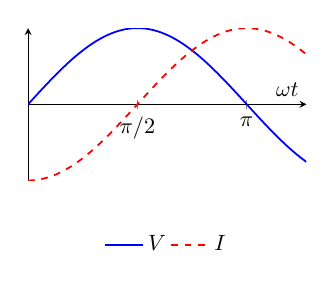
\begin{tikzpicture}[scale=0.8]
    \begin{axis}[
        width=6cm, height=4cm,
        axis lines=middle,
        xtick={0, 1.57, 3.14},
        xticklabels={0, $\pi/2$, $\pi$},
        ytick=\empty,
        xlabel=$\omega t$,
        legend style={at={(0.5,-0.3)}, anchor=north, legend columns=-1, draw=none}
    ]
    \addplot[blue, thick, domain=0:4, samples=100] {sin(deg(x))};
    \addlegendentry{$V$}
    \addplot[red, dashed, thick, domain=0:4, samples=100] {sin(deg(x)-90)};
    \addlegendentry{$I$}
    \end{axis}
\end{tikzpicture}
\end{answerdiagram}

\keyword{Equation:} $V = L \times \frac{dI}{dt}$
\end{solutionbox}

\begin{mnemonicbox}
\mnemonic{VLIC: Voltage Leads current by 90 In inductor Circuit}
\end{mnemonicbox}

\questionmarks{2(c) OR}{7}{Define phase voltage, line voltage, phase current and line current for 3-phase AC. (i) Calculate the line voltage for star (Y) connection if the phase voltage is 100V. Also find the line current for star (Y) connection if the phase current is 5A (ii) Calculate the line voltage for delta ($\Delta$) connection if the phase voltage is 100V. Also find the line current for delta ($\Delta$) connection if the phase current is 5A.}

\begin{solutionbox}
\textbf{Answer}:

\begin{center}
\captionof{table}{3-Phase Definitions}
\begin{tabulary}{\linewidth}{|L|L|}
\hline
\textbf{Term} & \textbf{Definition} \\ \hline
\textbf{Phase Voltage} & Voltage across a single phase element \\ \hline
\textbf{Line Voltage} & Voltage between any two lines \\ \hline
\textbf{Phase Current} & Current flowing through a phase element \\ \hline
\textbf{Line Current} & Current flowing through a line \\ \hline
\end{tabulary}
\end{center}

\textbf{Star (Y) Connection:}
\begin{itemize}
    \item Line voltage = $\sqrt{3} \times$ Phase voltage = $\sqrt{3} \times 100 = 173.2$ V
    \item Line current = Phase current = 5 A
\end{itemize}

\textbf{Delta ($\Delta$) Connection:}
\begin{itemize}
    \item Line voltage = Phase voltage = 100 V
    \item Line current = $\sqrt{3} \times$ Phase current = $\sqrt{3} \times 5 = 8.66$ A
\end{itemize}

\begin{answerdiagram}{Star and Delta Connections}
\begin{circuitikz}[scale=0.7, transform shape]
    % Star
    \draw (0,0) node[anchor=north]{N} to[R, l=R] (0,2) node[anchor=south]{R};
    \draw (0,0) to[R, l=Y] (-1.73,-1) node[anchor=north]{Y};
    \draw (0,0) to[R, l=B] (1.73,-1) node[anchor=north]{B};
    \node at (0,-2.5) {Star Connection};

    % Delta
    \begin{scope}[xshift=5cm, yshift=-1cm]
    \draw (0,0) to[R, l=B] (4,0);
    \draw (0,0) to[R, l=R] (2,3.46);
    \draw (2,3.46) to[R, l=Y] (4,0);
    \node at (2,-1.5) {Delta Connection};
    \end{scope}
\end{circuitikz}
\end{answerdiagram}
\end{solutionbox}

\begin{mnemonicbox}
\mnemonic{SLIP: Star Line voltage is root3 Phase, In Delta Phase equals Line voltage}
\end{mnemonicbox}

\questionmarks{3(a)}{3}{State and explain Faraday's laws of electromagnetic induction with necessary diagram and equations.}

\begin{solutionbox}
\textbf{Answer}:

\keyword{Faraday's Laws:}
\begin{enumerate}
    \item \keyword{First Law:} When a conductor cuts magnetic flux, EMF is induced.
    \item \keyword{Second Law:} The magnitude of induced EMF is proportional to the rate of change of magnetic flux.
\end{enumerate}

\keyword{Equation:} $e = -N \frac{d\Phi}{dt}$

\begin{answerdiagram}{Faraday's Experiment}
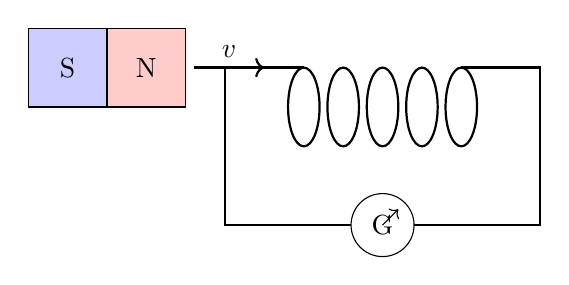
\begin{tikzpicture}
    % Coil
    \foreach \x in {0,0.5,1,1.5,2}
        \draw[thick] (\x,0) ellipse (0.2 and 0.5);
    \draw[thick] (0,0.5) -- (-1,0.5) -- (-1, -1.5) -- (3,-1.5) -- (3,0.5) -- (2,0.5);
    
    % Galvanometer
    \draw[fill=white] (1,-1.5) circle(0.4);
    \node at (1,-1.5) {G};
    \draw[->] (1,-1.5) -- (1.2,-1.3);

    % Magnet
    \draw[fill=red!20] (-2.5,0) rectangle (-1.5,1) node[midway]{N};
    \draw[fill=blue!20] (-3.5,0) rectangle (-2.5,1) node[midway]{S};
    \draw[->, thick] (-1.4, 0.5) -- (-0.5, 0.5) node[midway, above] {$v$};
\end{tikzpicture}
\end{answerdiagram}
\end{solutionbox}

\begin{mnemonicbox}
\mnemonic{FIRE: Flux change Induces Rapid EMF}
\end{mnemonicbox}

\questionmarks{3(b)}{4}{Define amplitude, frequency, time duration and RMS value for alternating quantity.}

\begin{solutionbox}
\textbf{Answer}:

\begin{center}
\captionof{table}{AC Definitions}
\begin{tabulary}{\linewidth}{|L|L|L|}
\hline
\textbf{Parameter} & \textbf{Definition} & \textbf{Formula} \\ \hline
\textbf{Amplitude} & Maximum value of the alternating quantity & $V_m$ \\ \hline
\textbf{Frequency} & Number of complete cycles per second & $f = 1/T$ \\ \hline
\textbf{Time Period} & Time taken to complete one cycle & $T = 1/f$ \\ \hline
\textbf{RMS Value} & Effective value, equivalent to DC causing same heating & $V_{rms} = 0.707V_m$ \\ \hline
\end{tabulary}
\end{center}

\begin{answerdiagram}{Waveform Parameters}
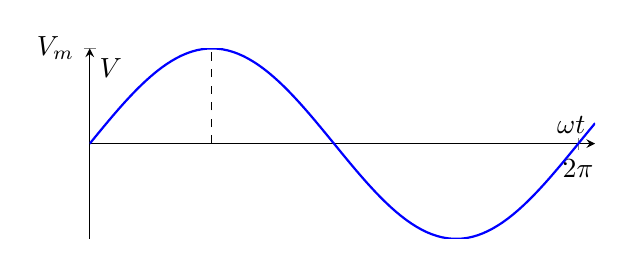
\begin{tikzpicture}
    \begin{axis}[
        width=8cm, height=4cm,
        axis lines=middle,
        xtick={0, 6.28},
        xticklabels={0, $2\pi$},
        ytick={1},
        yticklabels={$V_m$},
        xlabel=$\omega t$,
        ylabel=$V$
    ]
    \addplot[blue, thick, domain=0:6.5, samples=100] {sin(deg(x))};
    \draw[<->] (axis cs:0,-1.2) -- (axis cs:6.28,-1.2) node[midway, below] {Time Period $T$};
    \draw[dashed] (axis cs:1.57,0) -- (axis cs:1.57,1);
    \node at (axis cs:1.57,1.2) {Amplitude};
    \end{axis}
\end{tikzpicture}
\end{answerdiagram}
\end{solutionbox}

\begin{mnemonicbox}
\mnemonic{AFTR: Amplitude is peak, Frequency is cycles, Time is period, RMS is effective}
\end{mnemonicbox}

\questionmarks{3(c)}{7}{Explain self inductance and mutual inductance. (i) Find the self induction of the coil if total magnetic flux linked with the coil is 5 $\mu$Wb-turns for 2 A current given to the coil (ii) Find the self induction of the coil, if the parameters of the coils are as follows: number of turns is 10, relative permeability of the material used for coil is 3, length of the coil is 5 cm and cross sectional area of coil is 2 cm$^2$.}

\begin{solutionbox}
\textbf{Answer}:

\keyword{Self Inductance:} Property of a coil to oppose change in current through it by inducing EMF in itself.

\keyword{Mutual Inductance:} Property of one coil to induce EMF in another coil due to change in current in the first coil.

\textbf{Part (i):}
\begin{align*}
L &= \frac{\text{Flux Linkage}}{\text{Current}} \\
L &= \frac{5 \mu\text{Wb-turns}}{2 \text{A}} = 2.5 \mu\text{H}
\end{align*}

\textbf{Part (ii):}
\begin{align*}
L &= \frac{\mu_0 \mu_r N^2 A}{l} \\
L &= \frac{4\pi \times 10^{-7} \times 3 \times 10^2 \times 2 \times 10^{-4}}{5 \times 10^{-2}} \\
L &= 15.07 \mu\text{H}
\end{align*}

\begin{answerdiagram}{Self vs Mutual Inductance}
\begin{tikzpicture}
    % Self
    \draw[thick] (0,0) ellipse (0.2 and 0.5);
    \draw[thick] (0.5,0) ellipse (0.2 and 0.5);
    \node at (0.25, -1) {Self Inductance};
    \draw[->] (-0.5,0) -- (0,0) node[midway, above] {$I$};

    % Mutual
    \begin{scope}[xshift=4cm]
    \draw[thick] (0,0) ellipse (0.2 and 0.5);
    \draw[thick] (2,0) ellipse (0.2 and 0.5);
    \draw[->, wave] (0.5,0.2) -- (1.5,0.2) node[midway, above] {$\Phi$};
    \node at (1, -1) {Mutual Inductance};
    \end{scope}
\end{tikzpicture}
\end{answerdiagram}
\end{solutionbox}

\begin{mnemonicbox}
\mnemonic{SLIM: Self Linked with own flux, Induction Mutual between two coils}
\end{mnemonicbox}

\questionmarks{3(a) OR}{3}{Define dynamically induced EMF. Explain it with the help of necessary diagram and equation.}

\begin{solutionbox}
\textbf{Answer}:

\keyword{Dynamically Induced EMF:} EMF induced in a conductor due to relative motion between the conductor and magnetic field.

\keyword{Equation:} $e = B l v \sin\theta$
where $B$ is flux density, $l$ is length, $v$ is velocity.

\begin{answerdiagram}{Dynamic EMF}
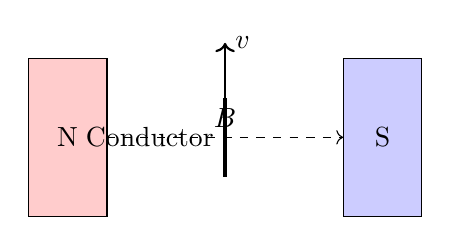
\begin{tikzpicture}
    \draw[fill=red!20] (0,0) rectangle (1,2) node[midway]{N};
    \draw[fill=blue!20] (4,0) rectangle (5,2) node[midway]{S};
    \draw[dashed, ->] (1,1) -- (4,1) node[midway, above] {$B$};
    
    \draw[ultra thick] (2.5, 0.5) -- (2.5, 1.5) node[midway, left] {Conductor};
    \draw[->, thick] (2.5, 1.5) -- (2.5, 2.2) node[right] {$v$};
\end{tikzpicture}
\end{answerdiagram}
\end{solutionbox}

\begin{mnemonicbox}
\mnemonic{MOVE: Motion Of conductor in magnetic field produces Voltage Effect}
\end{mnemonicbox}

\questionmarks{3(b) OR}{4}{Define cycle, Form Factor and Peak Factor for alternating quantity. Write the value of Form Factor and Peak Factor for sinusoidal alternating quantity.}

\begin{solutionbox}
\textbf{Answer}:

\begin{center}
\captionof{table}{AC Parameters}
\begin{tabulary}{\linewidth}{|L|L|L|}
\hline
\textbf{Term} & \textbf{Definition} & \textbf{Value (Sine)} \\ \hline
\textbf{Cycle} & One complete oscillation of an alternating quantity & - \\ \hline
\textbf{Form Factor} & Ratio of RMS value to average value ($V_{rms}/V_{avg}$) & 1.11 \\ \hline
\textbf{Peak Factor} & Ratio of maximum value to RMS value ($V_m/V_{rms}$) & 1.414 \\ \hline
\end{tabulary}
\end{center}
\end{solutionbox}

\begin{mnemonicbox}
\mnemonic{CFP: Cycle Finishes Pattern, Form Factor 1.11, Peak Factor 1.414}
\end{mnemonicbox}

\questionmarks{3(c) OR}{7}{State and explain Lenz's law. State and explain Fleming's right hand rule for generator. Find the energy stored in inductor having self inductance of 4 $\mu$H, if 3 A of current is flowing through the inductor.}

\begin{solutionbox}
\textbf{Answer}:

\keyword{Lenz's Law:} The direction of induced EMF is such that it opposes the change in magnetic flux that produces it.

\keyword{Fleming's Right Hand Rule:}
\begin{itemize}
    \item \textbf{Thumb:} Direction of motion
    \item \textbf{Forefinger:} Direction of magnetic field
    \item \textbf{Middle finger:} Direction of induced current
\end{itemize}

\keyword{Energy Calculation:}
\begin{align*}
E &= \frac{1}{2} L I^2 \\
E &= \frac{1}{2} \times 4 \times 10^{-6} \times 3^2 \\
E &= 18 \times 10^{-6} \text{ J} = 18 \mu\text{J}
\end{align*}

\begin{answerdiagram}{Fleming's Right Hand Rule}
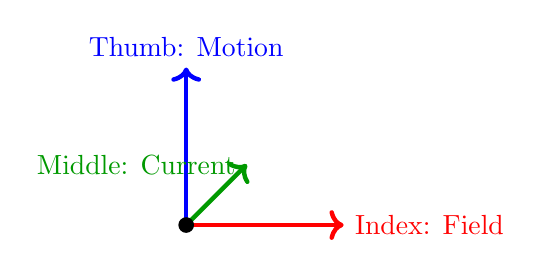
\begin{tikzpicture}
    \draw[->, ultra thick, blue] (0,0) -- (0,2) node[above] {Thumb: Motion};
    \draw[->, ultra thick, red] (0,0) -- (2,0) node[right] {Index: Field};
    \draw[->, ultra thick, green!60!black] (0,0) -- (0,0,-2) node[left] {Middle: Current};
    \node at (0,0) [circle, fill=black, inner sep=2pt] {};
\end{tikzpicture}
\end{answerdiagram}
\end{solutionbox}

\begin{mnemonicbox}
\mnemonic{LOF: Lenz Opposes Flux, Fleming Right for Generators}
\end{mnemonicbox}

\questionmarks{4(a)}{3}{Define PV cell. Explain the function of PV cell.}

\begin{solutionbox}
\textbf{Answer}:

\keyword{PV Cell:} A photovoltaic cell is a semiconductor device that converts light energy directly into electrical energy.

\keyword{Function:}
\begin{itemize}
    \item Absorbs photons from sunlight
    \item Creates electron-hole pairs
    \item Generates potential difference at p-n junction
    \item Produces DC electricity
\end{itemize}

\begin{answerdiagram}{PV Cell Operation}
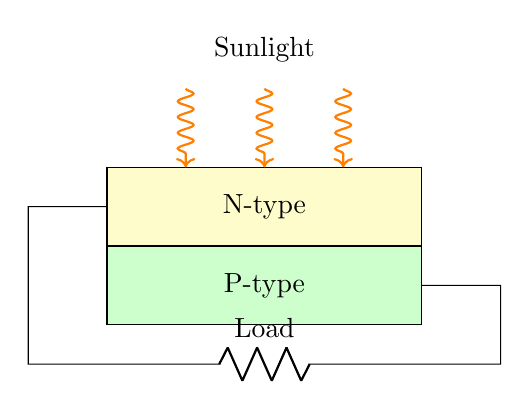
\begin{tikzpicture}
    \draw[fill=yellow!20] (0,1) rectangle (4,2) node[midway] {N-type};
    \draw[fill=green!20] (0,0) rectangle (4,1) node[midway] {P-type};
    \draw[->, decorate, decoration={snake, amplitude=1mm, segment length=2mm, post length=1mm}, thick, orange] (1,3) -- (1,2);
    \draw[->, decorate, decoration={snake, amplitude=1mm, segment length=2mm, post length=1mm}, thick, orange] (2,3) -- (2,2);
    \draw[->, decorate, decoration={snake, amplitude=1mm, segment length=2mm, post length=1mm}, thick, orange] (3,3) -- (3,2);
    \node at (2,3.5) {Sunlight};
    \draw (0,1.5) -- (-1,1.5) -- (-1,-0.5) to[R, l=Load] (5,-0.5) -- (5,0.5) -- (4,0.5);
\end{tikzpicture}
\end{answerdiagram}
\end{solutionbox}

\begin{mnemonicbox}
\mnemonic{PASE: PV Absorbs Sunlight, produces Electricity}
\end{mnemonicbox}

\questionmarks{4(b)}{4}{Explain the classification of green energy.}

\begin{solutionbox}
\textbf{Answer}:

\begin{center}
\captionof{table}{Green Energy Sources}
\begin{tabulary}{\linewidth}{|L|L|}
\hline
\textbf{Type} & \textbf{Source} \\ \hline
\textbf{Solar} & Sunlight (PV, Thermal) \\ \hline
\textbf{Wind} & Air currents (Turbines) \\ \hline
\textbf{Hydro} & Flowing water (Dams, Tidal) \\ \hline
\textbf{Biomass} & Organic matter (Biofuels) \\ \hline
\textbf{Geothermal} & Earth's heat \\ \hline
\end{tabulary}
\end{center}

\begin{answerdiagram}{Green Energy Classification}
\begin{tikzpicture}[
  level 1/.style={sibling distance=3cm},
  level 2/.style={sibling distance=1.5cm}
]
\node [gtu root] {Green Energy}
    child { node [gtu child] {Solar} }
    child { node [gtu child] {Wind} }
    child { node [gtu child] {Hydro} }
    child { node [gtu child] {Biomass} }
    child { node [gtu child] {Geothermal} };
\end{tikzpicture}
\end{answerdiagram}
\end{solutionbox}

\begin{mnemonicbox}
\mnemonic{SWHBG: Sun, Wind, Hydro, Biomass, Geothermal}
\end{mnemonicbox}

\questionmarks{4(c)}{7}{Draw and explain the block diagram of solar power system.}

\begin{solutionbox}
\textbf{Answer}:

\keyword{Components:}
\begin{itemize}
    \item \textbf{Solar Panel:} Converts sunlight to DC
    \item \textbf{Charge Controller:} Regulates battery charging
    \item \textbf{Battery Bank:} Stores energy
    \item \textbf{Inverter:} Converts DC to AC
    \item \textbf{Loads:} Consumes power
\end{itemize}

\begin{answerdiagram}{Solar Power System Block Diagram}
\begin{tikzpicture}[node distance=1.5cm, auto]
    \node [gtu block] (S) {Solar Panel};
    \node [gtu block, right=1cm of S] (C) {Charge\\Controller};
    \node [gtu block, below=1cm of C] (B) {Battery};
    \node [gtu block, right=1cm of C] (I) {Inverter};
    \node [gtu block, right=1cm of I] (L) {AC Load};
    
    \path [gtu arrow] (S) -- (C);
    \path [gtu arrow] (C) -- (I);
    \path [gtu arrow] (I) -- (L);
    \path [gtu arrow] (C) edge[bend left] (B);
    \path [gtu arrow] (B) edge[bend left] (C);
\end{tikzpicture}
\end{answerdiagram}
\end{solutionbox}

\begin{mnemonicbox}
\mnemonic{SCBIL: Solar Collects, Battery Inverts for Loads}
\end{mnemonicbox}

\questionmarks{4(a) OR}{3}{Define green energy, conventional energy and renewable energy.}

\begin{solutionbox}
\textbf{Answer}:

\begin{center}
\captionof{table}{Energy Definitions}
\begin{tabulary}{\linewidth}{|L|L|}
\hline
\textbf{Term} & \textbf{Definition} \\ \hline
\textbf{Green Energy} & Energy from eco-friendly sources with minimal impact \\ \hline
\textbf{Conventional Energy} & Traditional non-renewable sources like fossil fuels \\ \hline
\textbf{Renewable Energy} & Sources naturally replenished on human timescale \\ \hline
\end{tabulary}
\end{center}
\end{solutionbox}

\begin{mnemonicbox}
\mnemonic{GCR: Green is Clean, Conventional is Carbon, Renewable is Replenished}
\end{mnemonicbox}

\questionmarks{4(b) OR}{4}{Explain the need of green energy.}

\begin{solutionbox}
\textbf{Answer}:

\keyword{Need for Green Energy:}
\begin{itemize}
    \item \textbf{Environmental Protection:} Reduces pollution
    \item \textbf{Resource Conservation:} Saves fossil fuels
    \item \textbf{Energy Security:} Reduces import dependence
    \item \textbf{Economic Benefits:} Job creation
    \item \textbf{Sustainability:} For future generations
\end{itemize}
\end{solutionbox}

\begin{mnemonicbox}
\mnemonic{ERESS: Environment, Resources, Energy security, Savings, Sustainability}
\end{mnemonicbox}

\questionmarks{4(c) OR}{7}{Draw and explain the block diagram of wind power system with types of turbines.}

\begin{solutionbox}
\textbf{Answer}:

\keyword{Components:}
\begin{itemize}
    \item \textbf{Wind Turbine:} Converts wind to mechanical energy
    \item \textbf{Gearbox:} Increases speed
    \item \textbf{Generator:} Produces electricity
    \item \textbf{Controller:} Manages system
    \item \textbf{Transformer:} Steps up voltage
\end{itemize}

\keyword{Types:} HAWT (Horizontal Axis) and VAWT (Vertical Axis).

\begin{answerdiagram}{Wind Power System}
\begin{tikzpicture}[node distance=1.2cm, auto]
    \node [gtu block] (W) {Wind};
    \node [gtu block, right=0.5cm of W] (T) {Turbine};
    \node [gtu block, right=0.5cm of T] (G) {Gearbox};
    \node [gtu block, right=0.5cm of G] (Gen) {Generator};
    \node [gtu block, right=0.5cm of Gen] (C) {Controller};
    \node [gtu block, below=0.8cm of C] (Tr) {Transformer};
    \node [gtu block, left=0.5cm of Tr] (Grid) {Grid};
    
    \path [gtu arrow] (W) -- (T);
    \path [gtu arrow] (T) -- (G);
    \path [gtu arrow] (G) -- (Gen);
    \path [gtu arrow] (Gen) -- (C);
    \path [gtu arrow] (C) -- (Tr);
    \path [gtu arrow] (Tr) -- (Grid);
\end{tikzpicture}
\end{answerdiagram}
\end{solutionbox}

\begin{mnemonicbox}
\mnemonic{WGGTC: Wind, Gearbox, Generator, Transformer, Controller}
\end{mnemonicbox}

\questionmarks{5(a)}{3}{Explain the factors affecting the value of resistance of a resistor.}

\begin{solutionbox}
\textbf{Answer}:

\keyword{Factors Affecting Resistance ($R = \rho l/A$):}
\begin{itemize}
    \item \textbf{Length ($l$):} Directly proportional ($R \propto l$)
    \item \textbf{Area ($A$):} Inversely proportional ($R \propto 1/A$)
    \item \textbf{Temperature:} Increases for metals
    \item \textbf{Material ($\rho$):} Depends on resistivity
\end{itemize}
\end{solutionbox}

\begin{mnemonicbox}
\mnemonic{TLAM: Temperature, Length, Area, Material}
\end{mnemonicbox}

\questionmarks{5(b)}{4}{Define active power, reactive power, apparent power and power factor with the help of power triangle. Write their units.}

\begin{solutionbox}
\textbf{Answer}:

\begin{center}
\captionof{table}{Power Definitions}
\begin{tabulary}{\linewidth}{|L|L|L|}
\hline
\textbf{Term} & \textbf{Formula} & \textbf{Unit} \\ \hline
\textbf{Active Power (P)} & $P = VI \cos \phi$ & Watt (W) \\ \hline
\textbf{Reactive Power (Q)} & $Q = VI \sin \phi$ & VAR \\ \hline
\textbf{Apparent Power (S)} & $S = VI$ & VA \\ \hline
\textbf{Power Factor} & $\cos \phi = P/S$ & - \\ \hline
\end{tabulary}
\end{center}

\begin{answerdiagram}{Power Triangle}
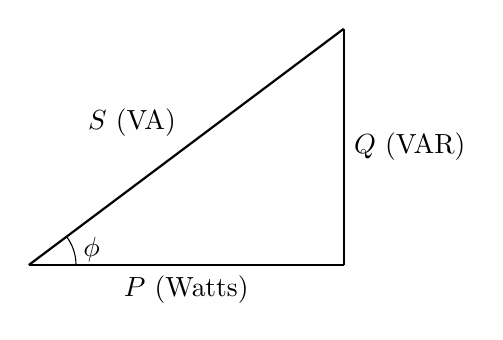
\begin{tikzpicture}
    \draw[thick] (0,0) -- (4,0) node[midway, below] {$P$ (Watts)};
    \draw[thick] (4,0) -- (4,3) node[midway, right] {$Q$ (VAR)};
    \draw[thick] (0,0) -- (4,3) node[midway, above left] {$S$ (VA)};
    \draw (0.6,0) arc (0:36.87:0.6) node[midway, right] {$\phi$};
\end{tikzpicture}
\end{answerdiagram}
\end{solutionbox}

\begin{mnemonicbox}
\mnemonic{ARSP: Active, Reactive, S-Apparent, Power Factor}
\end{mnemonicbox}

\questionmarks{5(c)}{7}{State and explain Kirchhoff's Voltage Law (KVL) and Kirchhoff's Current Law (KCL) with the help of circuit diagram.}

\begin{solutionbox}
\textbf{Answer}:

\keyword{KVL:} Algebraic sum of voltages in a closed loop is zero ($\sum V = 0$).

\keyword{KCL:} Algebraic sum of currents at a node is zero ($\sum I = 0$).

\begin{answerdiagram}{KVL and KCL}
\begin{circuitikz}[american, scale=0.8]
    % KVL
    \draw (0,0) to[V, l=$V_s$] (0,2) to[R, l=$R_1$] (2,2) to[R, l=$R_2$] (2,0) -- (0,0);
    \node at (1,-0.5) {KVL: $V_s - IR_1 - IR_2 = 0$};
    
    % KCL
    \begin{scope}[xshift=4cm]
    \node[circle, fill, inner sep=1.5pt] (N) at (0,1) {};
    \draw[<-] (N) -- (-1,1) node[left] {$I_1$};
    \draw[->] (N) -- (1,2) node[right] {$I_2$};
    \draw[->] (N) -- (1,0) node[right] {$I_3$};
    \node at (0,-0.5) {KCL: $I_1 = I_2 + I_3$};
    \end{scope}
\end{circuitikz}
\end{answerdiagram}
\end{solutionbox}

\begin{mnemonicbox}
\mnemonic{VCL: Voltage Closed Loop, Current Node Sum}
\end{mnemonicbox}

\questionmarks{5(a) OR}{3}{Write the difference between EMF and potential difference. Also write the difference between cell and battery.}

\begin{solutionbox}
\textbf{Answer}:

\begin{center}
\captionof{table}{Differences}
\begin{tabulary}{\linewidth}{|L|L|}
\hline
\textbf{EMF} & \textbf{Potential Difference} \\ \hline
Energy supplied per unit charge & Energy Consumed \\ \hline
Exists in open circuit & Exists in closed circuit \\ \hline
Cause of current & Effect of current \\ \hline
\end{tabulary}
\end{center}

\textbf{Cell vs Battery:} Cell is a single unit; Battery is a combination of cells.
\end{solutionbox}

\begin{mnemonicbox}
\mnemonic{ESOP: EMF Source, Potential Operating}
\end{mnemonicbox}

\questionmarks{5(b) OR}{4}{Write the relation between AC voltage and AC current for pure resistor, pure capacitor and pure inductor. Draw the vector diagram of AC voltage and AC current for pure resistor, pure capacitor and pure inductor. Also write the value of power factor for pure resistor, pure capacitor and pure inductor.}

\begin{solutionbox}
\textbf{Answer}:

\begin{center}
\captionof{table}{Component Comparisons}
\begin{tabulary}{\linewidth}{|L|L|L|L|}
\hline
\textbf{Component} & \textbf{Relation} & \textbf{Phase} & \textbf{PF} \\ \hline
\textbf{Resistor} & $V=IR$ & In Phase (0$^\circ$) & 1 \\ \hline
\textbf{Inductor} & $V=L(dI/dt)$ & $I$ lags $V$ by 90$^\circ$ & 0 (lag) \\ \hline
\textbf{Capacitor} & $I=C(dV/dt)$ & $I$ leads $V$ by 90$^\circ$ & 0 (lead) \\ \hline
\end{tabulary}
\end{center}

\begin{answerdiagram}{Vector Diagrams}
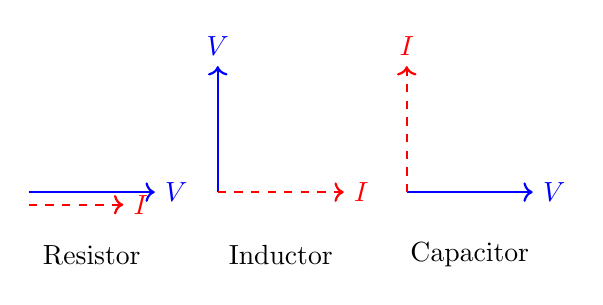
\begin{tikzpicture}[scale=0.8]
    % Resistor
    \draw[->, thick, blue] (0,0) -- (2,0) node[right] {$V$};
    \draw[->, thick, red, dashed] (0,-0.2) -- (1.5,-0.2) node[right] {$I$};
    \node at (1,-1) {Resistor};
    
    % Inductor
    \begin{scope}[xshift=3cm]
    \draw[->, thick, blue] (0,0) -- (0,2) node[above] {$V$};
    \draw[->, thick, red, dashed] (0,0) -- (2,0) node[right] {$I$};
    \node at (1,-1) {Inductor};
    \end{scope}

    % Capacitor
    \begin{scope}[xshift=6cm]
    \draw[->, thick, blue] (0,0) -- (2,0) node[right] {$V$};
    \draw[->, thick, red, dashed] (0,0) -- (0,2) node[above] {$I$};
    \node at (1,-1) {Capacitor};
    \end{scope}
\end{tikzpicture}
\end{answerdiagram}
\end{solutionbox}

\begin{mnemonicbox}
\mnemonic{RCI: Resistor Constant, Inductor lags, Capacitor leads}
\end{mnemonicbox}

\questionmarks{5(c) OR}{7}{Define temperature coefficient of material and write its unit. Explain the effect of temperature on resistance of conductor with the help of temperature coefficient of conductor.}

\begin{solutionbox}
\textbf{Answer}:

\keyword{Temperature Coefficient ($\alpha$):} The fractional change in resistance per degree change in temperature.
\keyword{Unit:} Per degree Celsius ($^\circ$C$^{-1}$).

\keyword{Effect on Conductors:}
\begin{itemize}
    \item Resistance increases with temperature (Positive $\alpha$)
    \item $R_2 = R_1 [1 + \alpha (T_2 - T_1)]$
\end{itemize}

\keyword{Effect on Semiconductors:} Resistance decreases (Negative $\alpha$).

\begin{answerdiagram}{Temperature Effect}
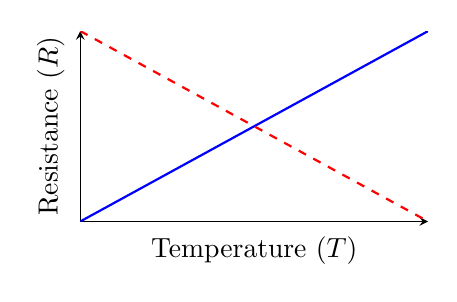
\begin{tikzpicture}
    \begin{axis}[
        width=6cm, height=4cm,
        axis lines=left,
        xlabel=Temperature ($T$),
        ylabel=Resistance ($R$),
        xtick=\empty, ytick=\empty
    ]
    \addplot[blue, thick, domain=0:10] {1 + 0.1*x} node[right] {Conductors (+$\alpha$)};
    \addplot[red, dashed, thick, domain=0:10] {2 - 0.1*x} node[right] {Semiconductors (-$\alpha$)};
    \end{axis}
\end{tikzpicture}
\end{answerdiagram}
\end{solutionbox}

\begin{mnemonicbox}
\mnemonic{TRIP: Temperature Raises resistance In Proportion}
\end{mnemonicbox}

\end{document}
